\documentclass[lang=cn,11pt,a4paper]{elegantpaper}
\usepackage{url}
\usepackage{booktabs}
\usepackage{multirow}
\usepackage{geometry}
\usepackage{longtable}
\usepackage{pdfpages}
\title{First Assignment}
\author{??? ??? ???}
% \usepackage[authoryear]{gbt7714}  % ??
\begin{document}
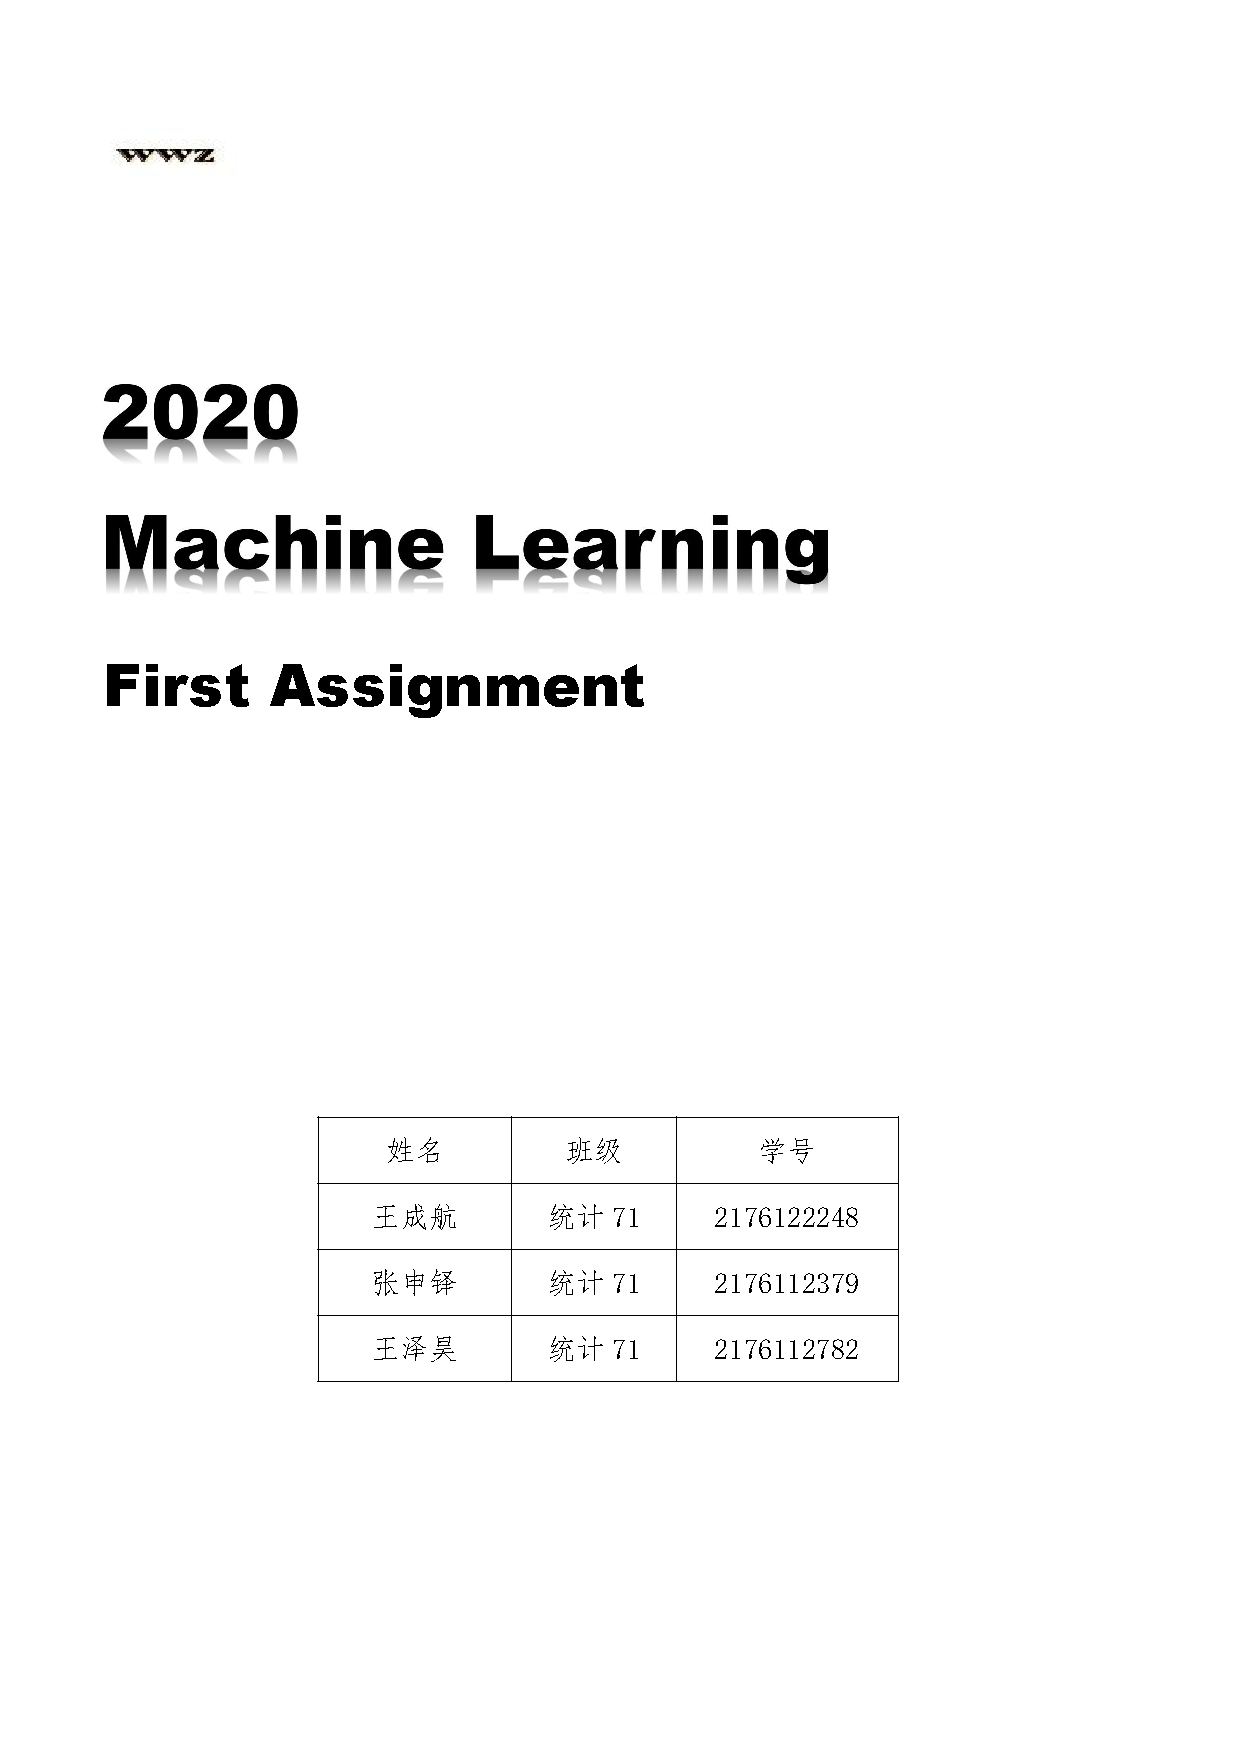
\includepdf[width=\paperwidth]{FM.pdf}
\newpage
\tableofcontents
\thispagestyle{empty}
\newpage
\pagenumbering{arabic}
\section{??}
\subsection{????????????}
\par ??20???, ?????????????????, ??????????, ????????????????. ????????????????????????, ??????????????????. IBM??????5???, ???Volume?Velocity?Variety?Value?Veracity, ???????????????????????. \figref{fig:data} ??????????????????????, ???????????????????????. ????????????????????????, ??, ????????????????????. 
\begin{figure}[htbp]
	\centering
	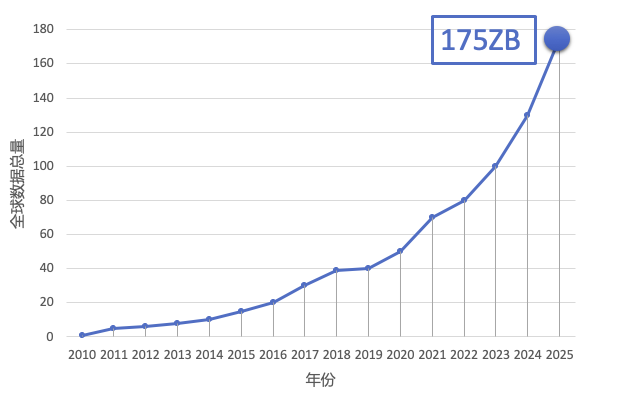
\includegraphics[width=0.45\textwidth]{Bigdata}
  	\caption{Rapid growth of data.\label{fig:data}}
\end{figure}
\par ???????????, ???????????,?????????????, ???????????????????????. ????????????, ????????????. ??????????, ??????????????????, ??Hadoop???????????????????????????. ??, ?? Caffe ? TensorFlow ??????????????, ????????????????????????????. ????????, ????????????. 
\par ?\figref{fig:data} ??, 2020?????????????50ZB, ????????????????????????, ????????, ????????????, ??????, ???????????, ???????????????????????????. ??????, ??????????????????( Data Technology, DT )??.
\begin{figure}[htbp]
	\centering
	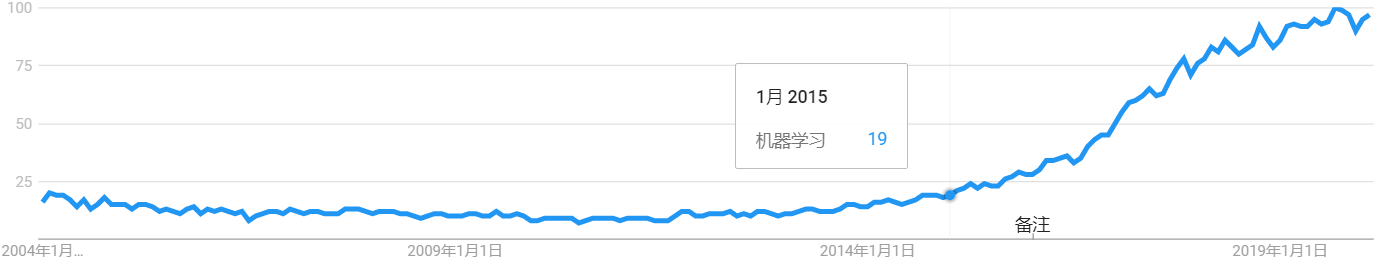
\includegraphics[width=0.85\textwidth]{GoogleTrend}
  	\caption{Google Trend about Machine Learning.\label{fig:GoogleTrend}}
\end{figure}
\par \figref{fig:GoogleTrend} ?????????????????????????\cite{GT}, ????, ?2015???, ??????????????, ??????????Google???DeepMind?????AlphaGo. AlphaGo???????????????????, ???????2015?3??????????????, ????3:1????????. ????, AlphaGo??????????????????. 
\par ??????, ??????2004????, ????Google?????2004????????????????????????????????????. ???, Facebook??????????????????????, ?????????, ??????????????????. ??????????????????, ?Alibaba?????, ?????????????????????, ???Alibaba????????????????????????????. ??2000????????????Tencent???????????????, ?QQ?????????, ??????, ????????????????, ???????????.
\par ??????????, ??????????????, ???????(\figref{fig:Brian} )???????????????, ?????????????????????; ??????????(\figref{fig:Machine} )?????????????????????????, ?????????, ?????????????. 
\begin{figure}[htbp]
	\centering
	\begin{minipage}[t]{0.45\textwidth}
	\centering
	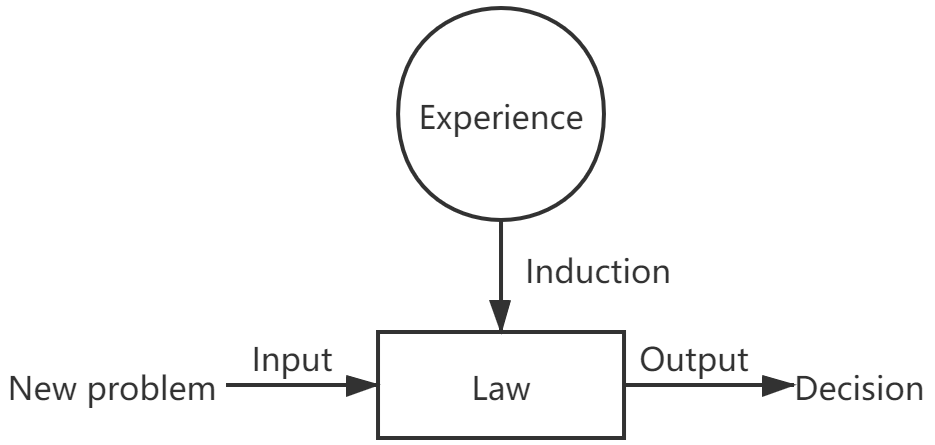
\includegraphics[width=1\textwidth]{Brian}
	\caption{How our brians learn.\label{fig:Brian}}
	\end{minipage}
	\begin{minipage}[t]{0.45\textwidth}
	\centering
	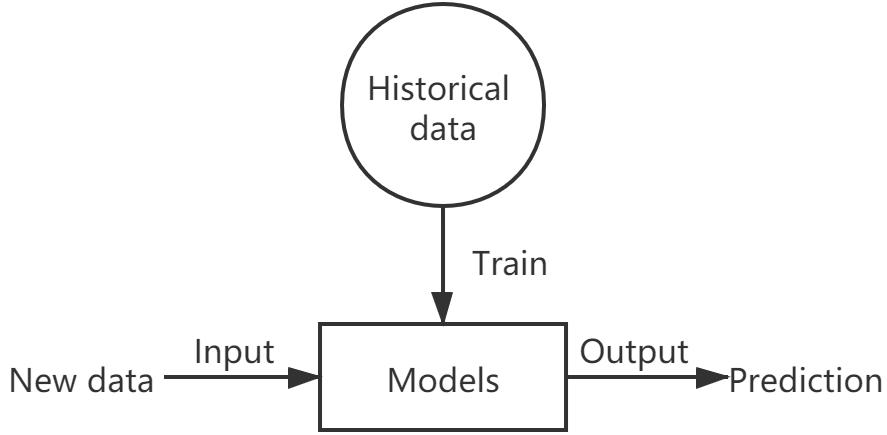
\includegraphics[width=1\textwidth]{Machine}
	\caption{How machines learn.\label{fig:Machine}}
	\end{minipage}
\end{figure}
\par ????????????????????, ???????????1952?IBM???Arthur Samuel?????????, ?????????????????, ????????\cite{AS1}\cite{AS2}. ???????, ????????????????????????????, ????????????????????, ?????????(\figref{fig:AI} ).
\begin{figure}[htbp]
	\centering
	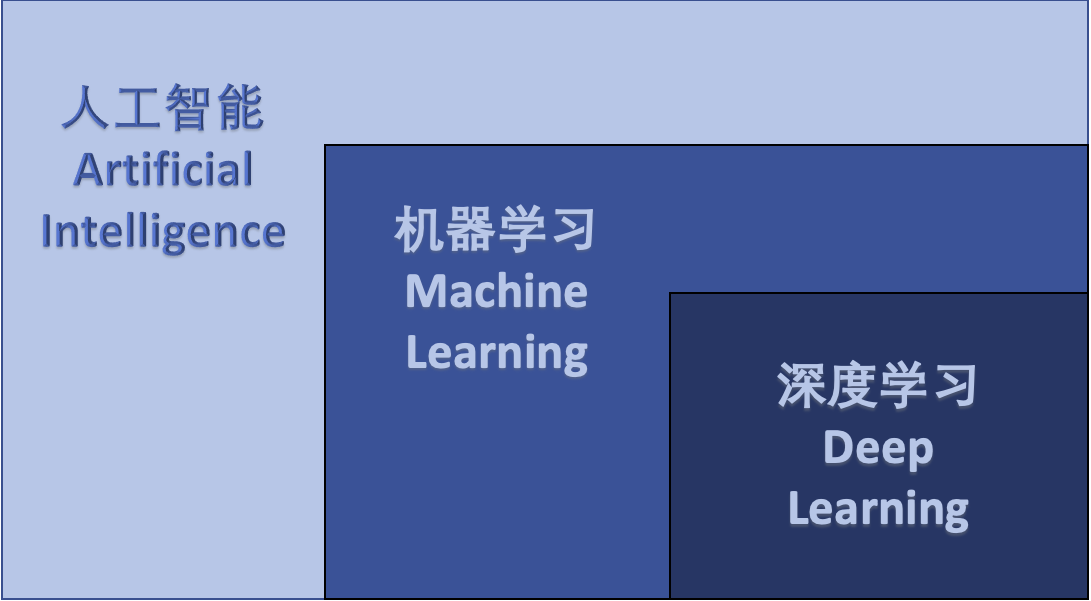
\includegraphics[width=0.5\textwidth]{AI}
  	\caption{AI, Machine Learning \& Deep Learning.\label{fig:AI}}
\end{figure}
\subsection{????}
\par ??????????1956????????\cite{Dartmouth}?????????, ????????????????, ???????????????????????????. ??, ??????????????????????????????. 
\par ???????????????????, ???????????Deeper Blue. ??????????($35^{80}$\cite{artic})??????, ?????????????????????????????????, ?Deeper Blue????????????????????. ?Deeper Blue??????, ???????, ???????????????. ???????????????????????????????. 
\par ???, ????????????????, ?????????????????????($250^{150}$\cite{artic}), ????????????????????, ??, ????????????????, ?????????.
\subsection{????}
\par 1950?, ??????Alan Turing????Computing machinery and intelligence???\cite{Turing2009}, .??, ?????????????????????????, ??????????: ?. 
\par ????????????, ?????????????????, ?????????????(\figref{fig:old} ). ???????, ?????????, ????????????????????????(\figref{fig:now} ). 
\begin{figure}[htbp]
	\centering
	\begin{minipage}[t]{0.45\textwidth}
	\centering
	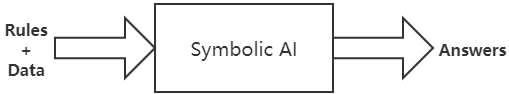
\includegraphics[width=1\textwidth]{Old}
	\caption{What Symbolic AI do.\label{fig:old}}
	\end{minipage}
	\begin{minipage}[t]{0.45\textwidth}
	\centering
	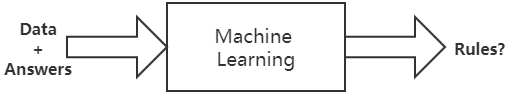
\includegraphics[width=1\textwidth]{Now}
	\caption{What ML do.\label{fig:now}}
	\end{minipage}
\end{figure}
\par ?????, ???????????????????????????????????. ????, ????????????????????, ??????????????, ?????????, ???????????. ????, ????????????????????AlphaGo Zero, ???????????????????. 
\subsection{????}
\par ???????????, ?????????????,????????????????????, ?????????????????????????????????, ???????????????, ????????????, ?????????, ???????????????. 
\begin{figure}[htbp]
	\centering
	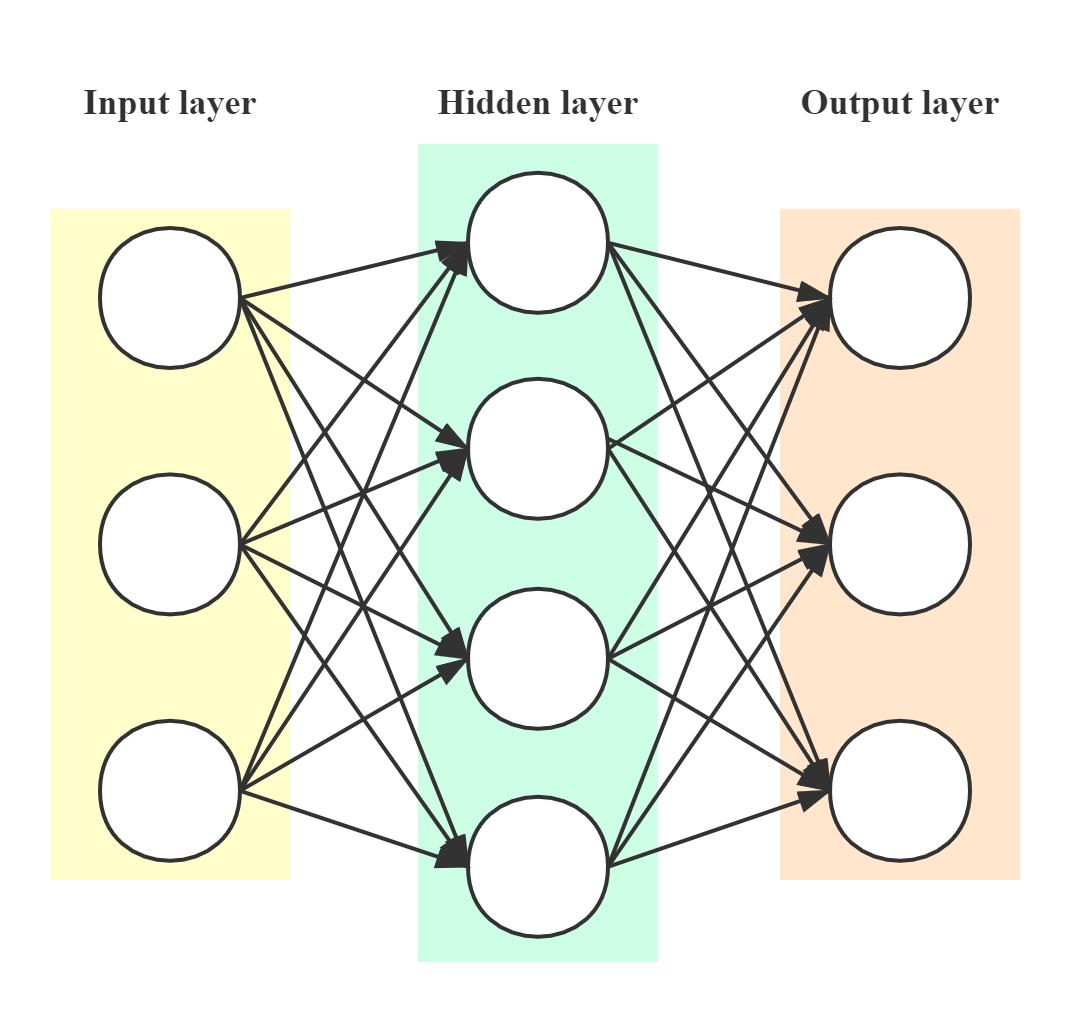
\includegraphics[width=0.4\textwidth]{DNN}
  	\caption{A three-layer full connected neural network\label{fig:DNN}}
\end{figure}
\par ????????????, ??????????????????????????????, \figref{fig:DNN} ???????????. ?????????????????????. ???????????, ??????????, ???????????????????????????????. ?????????????????, ????????????. ??????????????????\figref{fig:net} , ????????????????????????, ??????????.
\begin{figure}[htbp]
	\centering
	\hspace{-30pt}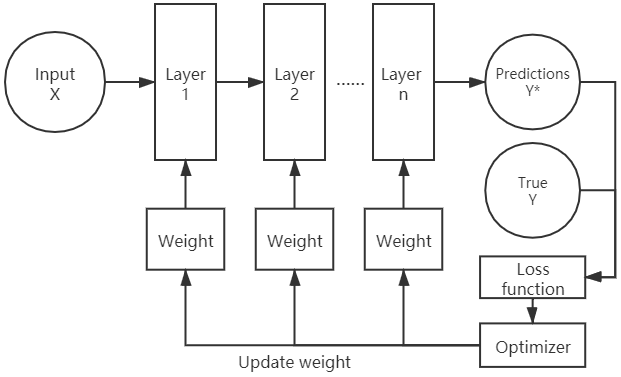
\includegraphics[width=0.5\textwidth]{Net}
  	\caption{The workflow of neural network ML.\label{fig:net}}
\end{figure}
\section{??????????}
\subsection{????}
\par ????????????, ?????????????????????????. 
\subsubsection*{20??50 - 70??}
\par ??, ????????????, ????????????????, ?????: A. Newell?H. Simon????????( Logic Theorist )???????????????( General Problem Solving )???, ????????????????. 
\par 20??70??????, ?E.A.Feigenbaum?????, ??????????????, ?????????. E.A.Feigenbaum?????????. ????, ?????????, ????????????????????, ???????????????.????1950?????, ??????????????, ?????????????????????????????????????????????????????????????????.
\subsubsection*{20??80??}
\par 1986?, ????Machine Learning???1989?, ????????Artificial Intelligence?????????20??80????????????????, ??, ???????????????????.
\par ???????????????????, ??????, ???????. ??, ????????????????????????????, ????????????????, ??????????????, ????????????????, ????????.
\subsubsection*{20??90??}
????????????????, ?????????SVM???????.???????????????????, ???????????, ???(kernel trick)????????????, ???????????????.

\vspace{10pt}
\begin{figure}[htbp]
	\centering
	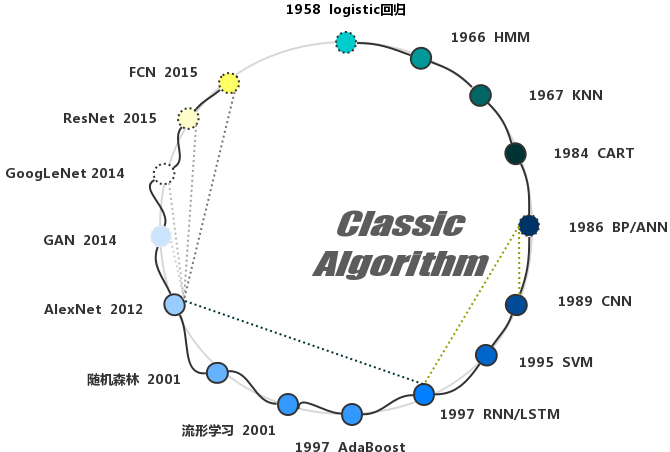
\includegraphics[width=0.6\textwidth]{SF}
  	\caption{The evolution of the algorithm.\label{fig:SF}}
\end{figure}

\vspace{-20pt}
\subsubsection*{21??}
??????????????, ??????????????????, ?????????????, ???????????????????????????, ???????????????, ?????????. ??, ??????????, ?????????????????, ????????????.
\par \figref{fig:SF} ?????????????????.
\subsection{????}
\par ?????????????????, ???????????????, ????????????????????????????????????????????????????????????????????????.
\paragraph{????}?????????????????????????????????????????????, ????????????, ????????. ????????????????, ?????????????????, ???????????????, ????????????????????????. ?????????????????????????????????, ???????????, ???????????????????????.
\paragraph{????}?????????????????, ?????????????. ??????????????????????. ????????????, ??????????????, ?????????????, ???????????????, ???????. ?????APP?????????????????????????????????.
\paragraph{???????}??????????????????, ???????Google????????. ?????????????????. ??????????????????????????, ????????????, ???????????, ??????. ???????????????, ??????????????????. ??????, ?????????????????????, ????????????????. ?????????, ????????????, ??????????, ????????????????????????????????, ?????????????????, ????????????????????. 
\subsection{Uber?????}
???Uber??????????, 2017?9?, Uber????????????--Michelangelo. ??Michelangelo, Uber??????????. 
\subsubsection*{Uber Eats} 
??Michelangelo, Uber Eats????????????????????????,??????????. 
\subsubsection*{????}
Uber??????????????????, ?????????Uber???????. Uber???????????, ?????????????????????. ??, ???????( surge  pricing )????, ????Uber????????. ?????, ??????????????????????????, ???, ???????????. ???????????????, ?????????. ???????, ????????, ???????, ?????????. 
\subsubsection*{??????( ETAs )}
?????, ????????????????. ??????????????????, ?????????????????, ??????????. 

Uber?????????????????????, ??????????. ??????????????????. ???????????????????????????, ????????????. ????????????????, Uber ??????????????????, ??????, ??????????????50\%??. 

\section{???????????}
\par ??????????????????????????????????. 
\par ??????????, ??????????????????, ??????????????????. ?????????????????. ????????????, NLP, ????????????????????????. ????????????????????????, ?????????????????. 
\par ?????, ?????????????????????, ??????????. ????????????????????, ????, ??????????????????????????????. ?????????????????????????????????????????????.
\par ???????????????????????????????????. ??????. ????????????????????????????????????????????. ?????????????????????????????.
\subsection{??????-????}
\par ?????????, ??????????????????$f:\mathcal X \to \mathcal Y$, $\mathcal X \subset \mathbb R^m, \mathcal Y \subset \mathbb R^n$, ?????????????????????????????????, ???????????????????$x\in \mathcal X$, ??????, ??????????????????????$y\in \mathcal Y$, ?????????????????, ???????????????????????. ????????????????????, ???????, ????????????????.
\par ??????, ????????????????????????????????, ?????????????????????????, ???????Deep ReLU Network(????????????). 
?????????????, ??????????????????????????????????????????, ????$E\in \mathcal X \times \mathcal Y$??????$||f(x)-y||^2_2, (x,y)\in E$???????, ????????????????????????. ?????????????????????$\mathcal X$???????$\mathcal Y$?????, ??????????????????????????. ????????, ??????????????????, ??????????????????????\cite{Goldberg1992}.
\par ???????????????????????????????, ?????????????????????????????. ????????????????????, ????????????????????????????????, ???????????????. ??????????????????, ???????????????????????????????. ??????????, ?????????????????????????????????????????????. ??????????????, ????????????????.
\par ????????????????????????????????\cite{Candes2010} , ????????????????????. 
\subsection{???????-????}
\par ????, ???????????????$A\in \mathbb{R}^{n_1\times n_2}$, ???????????????????????? ?????????????, ???????????????????. ????????????????????. ???????????????????????????\cite{Candes2010}??????????????\cite{Eriksson2012}, ?????????????. ???????????????, ?????????????\cite{Candes2009}.
\par ?????????????????????????????, ????????????????????????\cite{Candes2010}. ??????$A$????????????????????, ???$X_{i,j}$???i????j????????, ??$rank(X)=r, r<<n$. ????????$A$?????, ????????????????????????. ????????????????????????????????m?. ????????????$Y\in \mathbb{R}^{m\times n}$,
\begin{equation}
	Y_{ij}:=\delta_{ij}X_{ij}, \quad \delta_{ij} \sim \text{Ber}(p) \text{ are independent}, \quad p=\dfrac{m}{n_1n_2}
\end{equation}
\par ????????????????, ????????????$\hat{X}$????$||\hat{X}-X||_F$??. (???????????$X$??????????$Y$?????).
\par ?????????????????????$p^{-1}Y$???r??????\cite{Recht2011}. ????r???????
\begin{equation}
	p^{-1}Y_r=\frac{1}{p}\sum_{i=1}^r s_i u_i \otimes v_i, s_i \in \mathbb R, u_i \in \mathbb R^{n_1}, v_i\in \mathbb R^{n_2}
\end{equation}

????$Y$??????r???????, ????? 
\begin{equation}
||Y_r-Y||=\min_{rank(Y')\leq r}||Y-Y'||,
\end{equation}
??? $||\cdot||$ ????????, ??F???2-??, ??????????????????????. ?????$\hat X$???????????????, ???????????????????????????
\par ??????????, ???????????, ??$m\geq ctn\log n,\, n=\max\{n_1,n_2\}$???, ???????(????$1-(2n)^{1-t}$)??????????
\begin{equation}
	\dfrac{1}{n}||\hat X -X||_F\leq C\sqrt{\dfrac{tn\log n}{m}}||X||_{\infty},
\end{equation}
 ??$t>1$, $c,C$???????$X$???\cite{Recht2011}. 
 
 \par ??????, ??????????, ????????????($A$????????????????), ??????????????, ??$m\geq C n^{1.2} \log(n)$, ???????(??$1-cn^{-3}\log n$), ?????????$A$, ??$c,C$???????$X$???\cite{Candes2009}. ????, ???????????, ???Completion???????, ??????????????????????(???$\log n$)\cite{Candes2010}.
\par ???????????????????????????, ???????????????. ????????????????????????????. ???????, ??????????????????????????, ???????????????????????. 
\par ????????????????????????, ??????????????????????????????????????. ????????????????????????????, ?????????Expressiveness\cite{Yarotsky2017}???????Empirical Process\cite{Vapnik1994}?????, ????????????????????????????????????????????????.
\section{????????}
????????????????????, ??????????????????, ??????????????????????. \figref{fig:buzhou} ????????????.
\begin{figure}[htbp]
	\centering
	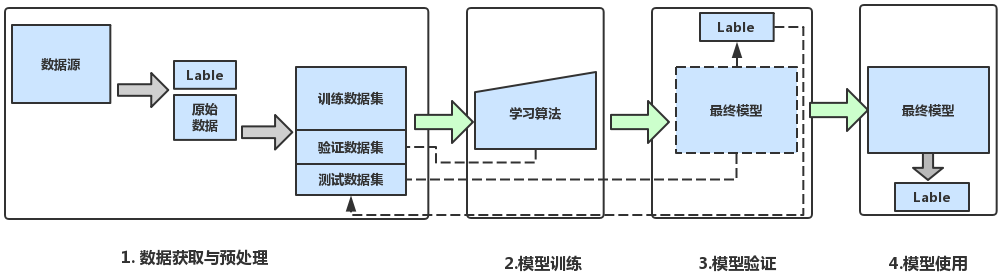
\includegraphics[width=0.9\textwidth]{555}
  	\caption{Procedure of Machine learning.\label{fig:buzhou}}
\end{figure}
\subsection{????????}
?????????????????, ???????????????????, ???????, ???????????????????. ???????????????????????. ????????, ?????????????????????????, ??????, ????, ?????????????????????.

??, ???????, ???????????????, ????????????????. ????????????????, ????????????, ????????????, ????????????????????????. ????????????????, ????????????????????????, ???????????????, ???????????. 
\subsection{?????}
????????, ????????????????, ?????????????( ???? )?????, ???????. 
\paragraph{?????}?????????????????????.
\paragraph{????( ???? )}?????????????????.
\paragraph{????}?????????????????????????????. 
\paragraph{???}??????????????????, ?????????????????, ?????????????????????????????k?????????. ?????????????????. ????????????????????????????.

?????????, ???????????????????. 
\subsection{?????}
\par ?????????, ??????????????????. ????????????, ????????????????????????F1???ROC?.
\subsection{???????}
\par ??????????????????.
\section{?????????}
\par ?????????????, ???????????, ???????????.
\subsection{??????????}
??????????????????????????????????. ????, ??????????????, ????????????????, ????????????????, ????????????. 
\begin{figure}[htbp]
	\centering
	\hspace{45pt}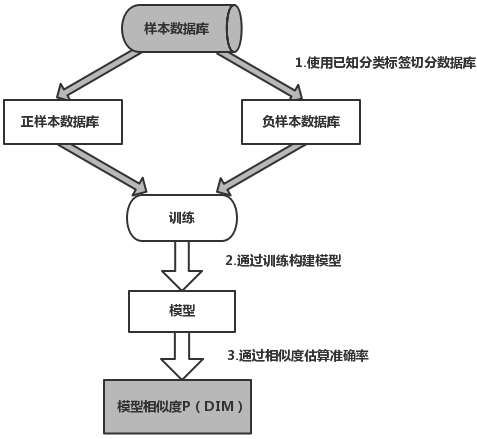
\includegraphics[width=0.4\textwidth]{SL}
  	\caption{Workflow of supervised learning.\label{fig:SL}}
\end{figure}
\subsubsection*{????}
??????????????????, ??????????????, ?????????. ?????????????????, ??????????, ????????, ????????????. ????????????????????????????????????????????. ??????????????????, ????, ???????????. ??????????????????????????, ????????, ???????????????????. ????????\figref{fig:SL} ??. 
\subsubsection*{?????}
???????????????????????. ???????????????????, ?????????????????????, ????????????????????. ????????????????????????????????, ????????????????????. ???????, ??????????????????????, ????????????. ???????????, ????????????????????, ????????????????????. ???????????Apriori???KMeans???????( random forest )??????( principal component analysis )?. 

\subsubsection*{?????}
???????????????????, ??????????????????????????????????, ????????????????????. ????????????, ???????????????????. ??????????????????, ????????????????. ?????( Graph inference )?????????????( Laplacian SVM )?. 
\subsubsection*{????}
??????????????????, ???????????. ?????????????, ??????????????????. ?????????????????????????????.????????, ????????????, ????????, ????????????????????. ??????, ???????????, ????????????. ?????????????????????. ??????Q-Learning???????( Temporal difference learning ). 
\subsection{??????????}
\subsubsection*{??}
???????????????????. ???????????????????????, ?????????????. ???????????????????????, ?????????????????????????. 
\subsubsection*{??}
??????????????????????????????. ?????????????????, ?????????????????, ??????????. ??????, ???????????, ??????????????, ???????????????. ??????KMeans?LDA?. 
\subsubsection*{??}
????????????????????, ???????, ??????????. ??????????????, ??????????????. ????????. 
\subsubsection*{??}
?????, ???????????????????????????????, ????????????????????????????????????. ??, ?????????????, ????????????, ??????????????????. ??, ????????, ?????????????????. ???????????????????????, ???????????. ??????????????????. ???????, ?????????????????, ?????????, ????????????, ???????????. 

\section{?????????}

?????????????, ????????????????????????, ???????????????. ????????????????. ????????????????????????????? ???????????????????, ??Hinton?LeCun?2019?????????????????????.

??Hinton??\cite{Youtube}?????????, ????????, ???????????????????????????. ???????????????????????, ???????????, ?????, ?????????????. \cite{kosiorek2019stacked}

??????????????????, ?????????, ?????????????. ???????????????????????????????. ????????????????????, ?????????????????, ????????????. 

???????????, ???????????????. ???????????????????????????????????(??????)?????. ????????????????????, ?????????, ?????????????????????????. ???????????????????????????. ???????????, ?????????????.

LeCun?????????????????????. ??????????????????????????????????, ????????. ??????????????????, ?????????. ???????????????????????????, ???????. ????????????, ????????, ?????????, ?????????????????????.

??, ???????????, ????????????????????????????????????????????????????????????? ???????????.
\newpage
\appendix
\pagenumbering{Roman}
\section{?????????}
\begin{longtable}[c]{|l|l|l|}
	\hline
	??    & ??                                                                                                               & ??                                                                      \\ \hline
	\endfirsthead
	%
	\endhead
	%
	\hline
	\endfoot
	%
	\endlastfoot
	%
	1949? & Hebb????????Hebb????                                                                                             & \multirow{6}{*}{\begin{tabular}[c]{@{}l@{}}?????\\ ????\end{tabular}}   \\
	1950? & Alan Mathison Turing???????                                                                                      &                                                                         \\
	1956? & \begin{tabular}[c]{@{}l@{}}John McCarthy, Cloude Shannon??\\ ??????? ( Artificial Intelligence )?\end{tabular}   &                                                                         \\
	1957? & \begin{tabular}[c]{@{}l@{}}Frank Rosenblatt???????\\ ???????????? (The Perceptron )\end{tabular}                 &                                                                         \\
	1956? & \begin{tabular}[c]{@{}l@{}}Arthur Samuel????????( Machine Learning )???, \\ ???????????????????????\end{tabular} &                                                                         \\
	1967? & k???????( KNN )??                                                                                                &                                                                         \\ \hline
	\multicolumn{3}{|c|}{??????????20??60?????70???}                                                                                                                                                   \\ \hline
	1980? & \begin{tabular}[c]{@{}l@{}}???????( CMU )???\\ ????????????\end{tabular}                                         & \multirow{4}{*}{\begin{tabular}[c]{@{}l@{}}?????\\ ????\end{tabular}}   \\
	1984? & Breiman??????????( CART )                                                                                       &                                                                         \\
	1986? & ?????\emph{Machine Learning}??                                                                                          &                                                                         \\
	1986? & \begin{tabular}[c]{@{}l@{}}Rumelhart?McClelland??????\\ ??BP????\end{tabular}                                    &                                                                         \\ \hline
	1989? & \begin{tabular}[c]{@{}l@{}}Yann LeCun???????????\\ ??????( CNN )??????\end{tabular}                              & \multirow{6}{*}{\begin{tabular}[c]{@{}l@{}}???????\\ ????\end{tabular}} \\
	1995? & Vladimir Vapnik???????( SVM )                                                                                   &                                                                         \\
	1995? & Freund?schapire??? AdaBoost??                                                                                    &                                                                         \\
	1997? & ??????( RNN )??                                                                                                  &                                                                         \\
	2000? & \begin{tabular}[c]{@{}l@{}}??????( Manifold Learning )?\\ \emph{Science}????, ??????Isomap?LE?PCA\end{tabular}           &                                                                         \\
	2001? & Breiman??????( Random Forest )                                                                                  &                                                                         \\ \hline
	2006? & \begin{tabular}[c]{@{}l@{}}Hinton???\emph{Science}??????\\ ???????????\end{tabular}                                     & \multirow{7}{*}{\begin{tabular}[c]{@{}l@{}}???????\\ ????\end{tabular}} \\
	2010? & Leslie Valiant?PAC???????                                                                                        &                                                                         \\
	2011? & Judea Pearl???????????                                                                                           &                                                                         \\
	2012? & \begin{tabular}[c]{@{}l@{}}Hinton?????????????\\ AlexNet??????????????\end{tabular}                              &                                                                         \\
	2014? & Lan.J.Goodfellow????GAN                                                                                          &                                                                         \\
	2017? & AlphaGo????                                                                                                      &                                                                         \\
	2019? & \begin{tabular}[c]{@{}l@{}}Geoffrey E Hintion?Yann LeCun?Yoshua Bengio\\ ????????????????\end{tabular}           &                                                                         \\ \hline
	\end{longtable}
\newpage
\nocite{*}

% ???????????( ??? ), ????????, ????????( ?? unsrt, plain ?? ). 
\bibliographystyle{unsrt}
\bibliography{wpref}

\end{document}
